%%
%% Copyright 2007-2020 Elsevier Ltd
%%
%% This file is part of the 'Elsarticle Bundle'.
%% ---------------------------------------------
%%
%% It may be distributed under the conditions of the LaTeX Project Public
%% License, either version 1.2 of this license or (at your option) any
%% later version.  The latest version of this license is in
%%    http://www.latex-project.org/lppl.txt
%% and version 1.2 or later is part of all distributions of LaTeX
%% version 1999/12/01 or later.
%%
%% The list of all files belonging to the 'Elsarticle Bundle' is
%% given in the file `manifest.txt'.
%%
%% Template article for Elsevier's document class `elsarticle'
%% with harvard style bibliographic references

%\documentclass[preprint,12pt,authoryear]{elsarticle}

%% Use the option review to obtain double line spacing
%% \documentclass[authoryear,preprint,review,12pt]{elsarticle}

%% Use the options 1p,twocolumn; 3p; 3p,twocolumn; 5p; or 5p,twocolumn
%% for a journal layout:
%% \documentclass[final,1p,times,authoryear]{elsarticle}
%% \documentclass[final,1p,times,twocolumn,authoryear]{elsarticle}
%% \documentclass[final,3p,times,authoryear]{elsarticle}
%% \documentclass[final,3p,times,twocolumn,authoryear]{elsarticle}
%% \documentclass[final,5p,times,authoryear]{elsarticle}
 \documentclass[final,5p,times,twocolumn,authoryear]{elsarticle}

%% For including figures, graphicx.sty has been loaded in
%% elsarticle.cls. If you prefer to use the old commands
%% please give \usepackage{epsfig}

%% The amssymb package provides various useful mathematical symbols
\usepackage{amssymb}
%% The amsthm package provides extended theorem environments
%% \usepackage{amsthm}

%% The lineno packages adds line numbers. Start line numbering with
%% \begin{linenumbers}, end it with \end{linenumbers}. Or switch it on
%% for the whole article with \linenumbers.
%% \usepackage{lineno}


\begin{document}

\begin{frontmatter}

\title{WE NEED A TITLE HEERE ???}

\author[first]{André Costa}
\author[second]{Celso Ribeiro}
\author[third]{David Mendes}
\affiliation{organization={ISCTE – Instituto Universitário de Lisboa},
            country={Portugal}} % Title page setup

\begin{abstract}
%% Text of abstract
This article aims to summarize the approach and results of \cite{Stacking}, in which the authors explore employing stacking, boosting, and blending machine learning algorithms to predict student performance in large-scale assessments based on a wide range of predictors and compare their performance.
\end{abstract}

\begin{keyword}
PISA \sep Machine learning \sep Stacking \sep Boosting \sep Blending \sep Ensemble
learning
\end{keyword}

\end{frontmatter}

%\tableofcontents

%% \linenumbers

%% main text

\section{Introduction}
\label{introduction}

\subsection{Business Understanding}
\label{sec:business_understanding}

Large‑scale international assessments such as the \textbf{Programme for International Student Assessment (PISA)} provide policy‑makers with uniquely comparable evidence on the cognitive skills of 15‑year‑olds.  Yet ministries and school leaders frequently lack timely, granular diagnostics that explain \emph{why} some learners underperform while others excel.  Our project addresses this gap by developing an AI‑based early‑warning model that flags students at risk of \textit{low achievement} in mathematics, science, and reading using the publicly released \textbf{PISA 2022 Student Questionnaire} micro‑data set.

The business—or, more precisely, educational policy—problem can be stated as follows:

\begin{quote}
  \emph{“Given a fixed budget for instructional support, how can education systems proactively target pedagogical and socio‑emotional interventions toward students most likely to obtain low PISA scores, thereby reducing grade repetition and narrowing equity gaps?”}
\end{quote}

Operationalising this question involves three goals:

\begin{enumerate}
  \item \textbf{Predictive analytics}: learn a mapping from student‑level contextual variables ($\mathbf{X}$) to performance deciles ($y$) that generalises across participating economies.
  \item \textbf{Actionable insights}: identify the subset of predictors with the \emph{strongest marginal contribution} to low performance, so interventions can be prioritised.
  \item \textbf{Benchmarking}: compare the risk profiles of repeating students against high performers, highlighting differences that may travel across national borders.
\end{enumerate}

\paragraph{Key findings to date.}
Exploratory correlation and feature‑importance screens on $\sim700$ candidate variables reveal four robust signals:

\begin{itemize}
  \item \textbf{Socio‑economic status (ESCS)} represents the largest single share of variance in low scores; a one‑decile drop in ESCS increases the probability of bottom-quartile performance by 6 to 8 pp.
  \item \textbf{Sense of school belonging} and \textbf{test‑skill confidence} together exert a comparable influence, especially on mathematics.
  \item \textbf{Late school entry} (age $>$ 7) and \textbf{grade repetition history} exhibit strong conditional correlations with poor science outcomes.
  \item Contrary to conventional belief, \textbf{time‑spent‑on‑homework} shows only a weak negative correlation once SES and self‑efficacy are controlled.
\end{itemize}

These empirical patterns motivate our choice of ensemble models (stacking, gradient boosting) that handle high‑dimensional, collinear, and partially missing data while producing interpretable feature importances.

\paragraph{Why cross‑country comparison matters.}
Although PISA is standardised, the institutional context in which 15‑year‑olds learn varies considerably:

\begin{description}
  \item[England] operates a \emph{comprehensive system} with Key Stages and externally set GCSE exams at age 16; grade repetition is rare and pupils can select specialised pathways post‑16.\footnote{\url{https://b28mathstutor.co.uk/how-the-english-school-system-works/}}
  \item[China–Shanghai (and other mainland provinces)] follows a \emph{high‑stakes, exam‑centric track}; the nine‑year compulsory cycle culminates in senior‑high entrance exams, and tutorial intensity is among the world’s highest.\footnote{\url{https://en.wikipedia.org/wiki/Education_in_China}}
  \item[Singapore] employs a differentiated but tightly sequenced route from Primary 1 through O‑Level/Integrated Programme, emphasising streaming and national examinations.\footnote{\url{https://en.wikipedia.org/wiki/Education_in_Singapore}}
  \item[Germany] divides students after Grade 4 into multiple secondary pathways (Gymnasium, Realschule, Hauptschule); grade repetition is relatively common and tracked.\footnote{\url{https://www.studying-in-germany.org/german-education-system/}}
  \item[United States] offers a largely \emph{comprehensive K–12} model governed by state standards and the Carnegie unit; social promotion policies reduce formal repetition but conceal skill deficits.\footnote{\url{https://en.wikipedia.org/wiki/Education_in_the_United_States}}
\end{description}

Recognising such systemic contrasts is essential: a “risk factor” identified in one jurisdiction (e.g.\ after‑school tutoring hours in Shanghai) may not be policy‑controllable in another (e.g.\ England, where after‑school tuition is privately financed).  Therefore, our modelling pipeline includes country‑specific fixed effects and studies interaction terms between student attributes and system‑level dummies.

\paragraph{What teaching strategies enhance reading performance?}
Insights from \textbf{PISA 2018} contextual data offer valuable evidence. According to the teacher questionnaire, strategies such as \emph{explicit reading instruction}, \emph{activating prior knowledge}, and \emph{engaging students in metacognitive practices} were correlated with higher reading performance. From the student perspective, respondents who reported frequent use of \emph{discussions about texts}, \emph{clarity in lesson structure}, and \emph{constructive feedback} also scored higher on average. Interestingly, while both teachers and students pointed to structured and cognitively activating instruction as beneficial, teachers tended to emphasize planning and scaffolding, whereas students highlighted motivation and classroom climate. This discrepancy reinforces the importance of triangulating perspectives in education data analytics.

\paragraph{Profiling students in vocational education tracks.}
Another avenue of investigation focuses on students enrolled in \textbf{vocational and professional training programs} as defined in PISA. Historically, these students perform lower in mathematics than those in general education tracks. Variables explaining this gap include reduced parental education, lower socio-economic status, and limited exposure to advanced mathematics content. However, over successive cycles of PISA (2012–2018), some countries have seen marginal gains for vocational-track students—particularly where applied mathematics and contextualised problem-solving were integrated into the curriculum. Our model incorporates program type as a categorical feature and enables interaction testing with SES, gender, and country-level effects to better understand these evolving patterns.


\paragraph{Success criteria.}
From a business‑value perspective, we deem the CRISP‑DM \emph{Business Understanding} phase complete when we can:

\begin{itemize}
  \item articulate the decision points (resource targeting, curriculum design) that model outputs will inform;
  \item translate model metrics into cost–benefit terms for ministries (e.g.\ reduction in misallocated tutoring hours per \$100k invested in data collection);
  \item outline ethical safeguards to prevent algorithmic bias against vulnerable groups.
\end{itemize}

Establishing this shared understanding with stakeholders ensures that the subsequent CRISP‑DM phases—Data Understanding, Data Preparation, Modelling, and Evaluation—remain anchored to actionable educational impact.


Building on this policy motivation, the empirical backbone of our work is the study by \cite{Stacking}, which exploits the same \textbf{PISA 2022 Student Questionnaire} micro‑data.  Their benchmark investigation compares three ensemble‑learning families—\emph{stacking}, \emph{boosting}, and \emph{blending}—for predicting mathematics, reading, and science scores.  Stacking aggregates the outputs of diverse base learners into a meta‑model, boosting trains learners sequentially so each iteration corrects the residuals of the previous one, while blending fits base models on a hold‑out validation set before meta‑aggregation.  \citeauthor{Stacking} report that stacking consistently yields the lowest error metrics (MAPE, MAE, MSE), a finding that motivates our own choice of stacked architectures for early‑warning classification.
\section{Methods}
%%\label{}

\subsection{Stacking}
Stacking is an ensemble learning technique developed by \cite{WOLPERT1992241} that combines several prediction models and uses their outputs as input for a next-level model (meta-model), aiming to improve overall prediction performance\cite{Stacking}. In the study \cite{Stacking}, the authors divide stacking into level 0 and level 1, where layer 0 refers to where the different models generate distinct predictions, and level 1 combines predictions of level 0. For level 0, some of the different models that could be used are DTs, NNs, SVMs, and kNN, in which the resulting predictions are then used and combined in layer 1, in order to improve the overall prediction \cite{WOLPERT1992241}, the authors choose to use ridge regression, which can be useful to avoid overfitting \cite{CUI2021107038}
\subsection{Boosting}
Because the dataset used in this study is composed of missing data, it is imperative to implement learners that deal with missing data, the boosting algorithms used were XGBoost, HGB, and LightGBM \cite{Stacking}
\subsection{blending}
Blending and stacking are both techniques used in ensemble learning that share similarities. The key difference between them is that in blending, the base learners are trained using predictions obtained from the validation set instead of directly from the training set\cite{Stacking}
\section{Results}
The study found that the stacking method produced the lowest error metrics (Mean Absolute Percentage Error (MAPE), Mean Absolute Error (MAE), Mean Squared Error (MSE)) for most countries compared to boosting and blending. Robust linear mixed-effects models indicated that stacking had significantly lower error metrics across all subjects as showed in \ref{fig:results}.

\begin{figure}
	\centering
	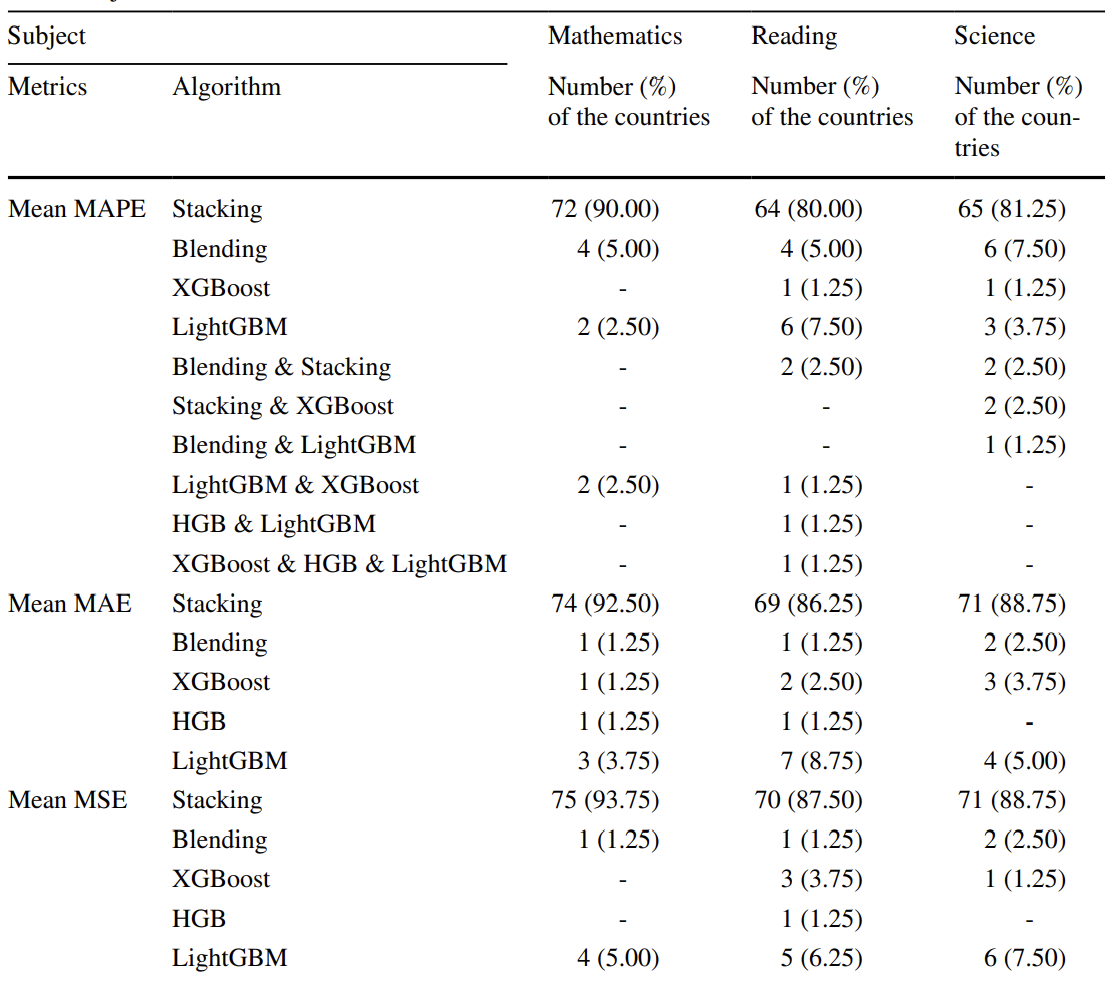
\includegraphics[width=0.4\textwidth]{figures/figure1}
	\caption{The Number (\%) of the countries exhibiting the lowest error values generated by each algorithm for all subjects \cite{Stacking}}
    \label{fig:results}
\end{figure}

\section{Conclusion}
The study \cite{Stacking} concludes that stacking is a favorable option for better performance, stable and accurate predictions based on evaluation with various metrics such as MAPE, MAE, MSE and RMSE where it obtained a significant metric score in all subjects compared to boosting and blending.
Due to this study only evaluating the PISA dataset, I think it would be interesting to evaluate it with other datasets to improve this analysis further


%% If you have bibdatabase file and want bibtex to generate the
%% bibitems, please use
%%
\bibliographystyle{elsarticle-harv}
\bibliography{main}

%% else use the following coding to input the bibitems directly in the
%% TeX file.

%%\begin{thebibliography}{00}

%% \bibitem[Author(year)]{label}
%% For example:

%% \bibitem[Aladro et al.(2015)]{Aladro15} Aladro, R., Martín, S., Riquelme, D., et al. 2015, \aas, 579, A101


%%\end{thebibliography}

\end{document}

\endinput
%%
%% End of file `elsarticle-template-harv.tex'.
